%\section{System Model}

The control system consists of three interconnected components as
illustrated in \figref{actual-system-diagram}:
\begin{enumerate}
\item The \emph{plant} is a continuous time LTI system of the form
\begin{align}
\dot{x}(t) & =A_{c}x(t)+B_{c}u(t)+w_{c}(t)\label{eq:plant-cont-model}
\end{align}
where $x\in\RR^{n}$ is the state, $u\in\RR^{m}$ is the control input,
and $w_{c}\in\RR^{n}$ is the process noise. 
\begin{comment}
The matrices $A_{c}$
and $B_{c}$ are system matrices of appropriate dimensions. Though
the process noise \end{comment}
Though $w_{c}$ is unknown, we assume that it belongs to
a known compact and convex constraint set $\WSet_{c}\subset\RR^{n}$.
%
\item The \emph{estimator} observes the plant output $y(t)=Cx(t)+v(t)$ (where $v$ is the output noise) and estimates the current state of the plant, which cannot be measured directly. %Here $C$ is the output matrix and $v$ is the output noise.
  Let $\hat{x}(t)$ denote the estimated state at time $t$ and $e(t)=x(t)-\hat{x}(t)$ be the error between the actual and estimated states. Note that $e(t)$ is unknown, however, depending on the characteristics of the estimation algorithm, it would be bounded. The upper bound $\sAccu(t)$ of the norm $\norm{e(t)}$, where $\norm{\cdot}$ is any vector norm, determines the \emph{accuracy} of the state estimation.
  The set of error vectors corresponding to an accuracy $\sAccu\geq0$ is denoted by $\ESet(\sAccu)\definedas\{e\in\RR^{n}\SuchThat\norm{e}\leq\sAccu\}$.  We assume that the estimator is an \textit{anytime algorithm} where there is a trade-off between the accuracy and the computation time.
  In particular, the more accurate the estimation is the longer it takes to compute, and conversely.
  The accuracy of the estimator, hence its computation time, can be adjusted online by changing its parameters or its algorithm.
  % The computation time, hence the accuracy of such an algorithm can be adjusted online.

%The accuracy of
%the estimator, hence its computation time, can be adjusted online
%by changing its parameters or its algorithm.

\item The \emph{controller} computes the control input for the plant as well as
adapts the estimator's accuracy to achieve a predefined control goal.
\end{enumerate}

\begin{figure}[tb]
	\centering
		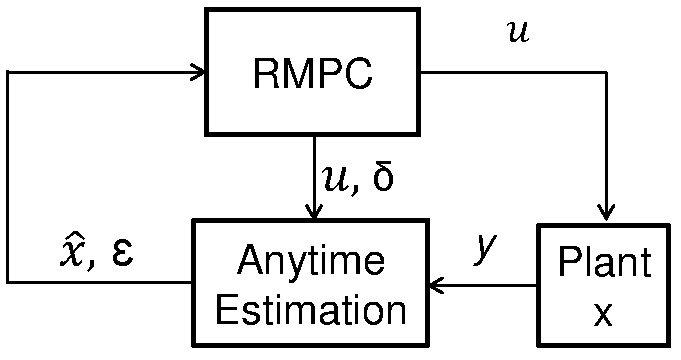
\includegraphics[width=0.40\textwidth,height=30mm]{figs/ControlFigure_scissored.pdf}
	\caption{Structure of the control and anytime estimation system.}
	\label{fig:actual-system-diagram}
\end{figure}



We consider a discrete time implementation of the controller and the estimator, in which the output $y(t)$ is sampled periodically at instants $t_{s,k}=kT$,
where $k\in\ZZplus$ and $T>0$ is a predefined sampling period.
The sampled output is fed to the estimator which computes the state
estimate $\hat{x}_{k}\definedas\hat{x}(t_{s,k})$ with the desired
accuracy $\sAccu[k]\definedas\sAccu(t_{s,k})$ determined by the controller
in the previous time step. The controller then uses this state estimate
to compute the control input $u_{k}$ as well as decide on the desired
state estimate's accuracy $\sAccu[k+1]$ for the next step. Let $\sDelay[k]$
be the worst-case total execution time of both the estimator and the
controller corresponding to the accuracy $\sAccu[k]$ of the state
estimation at time step $t_{s,k}$. We make the following theoretical
assumption of the state estimator.
\begin{assumption}
The estimation algorithm is given with a finite set of $p>0$ modes
(or options) $\Delta=\left\{ \left(\sDelay[i],\sAccu[i]\right)\right\} _{i=1}^{p}$;
each mode corresponds to a pair of time delay and estimation accuracy.
In each time step $k$, one of the estimation modes is selected, that
is $\left(\sDelay[k],\sAccu[k]\right)\in\Delta$.
\end{assumption}

This assumption means that in this paper we will not design nor analyze
the estimation algorithm; in other words, the estimator is a black-box
given to us with known characteristics. 

Furthermore, the control implementation
is subject to the following assumption.
\begin{assumption}
[Time-triggered actuation]The control actuation is delayed by $\sDelay[k]$,
\ie the control input computed by the controller is applied exactly
at the actuation instant $t_{a,k}=t_{s,k}+\sDelay[k]$.
\end{assumption}

The order of sensing\textendash{}computing\textendash{}actuating and
their timing are illustrated in the diagram in \figref{timing-diagram}.
We remark that in each step $k\geq0$, the estimation accuracy $\sAccu[k]$
and hence the delay $\sDelay[k]$ are already decided in the previous
step and known to the controller. The previous control input $u_{k-1}$
is still used until $t_{a,k}$ when the new control input $u_{k}$
is computed and applied by the controller. The controller also chooses
the next desired accuracy $\sAccu[k+1]$ and delay $\sDelay[k+1]$
to be used in the next step $k+1$. In the first step $k=0$, the
initial accuracy $\sAccu[0]$, the initial delay $\sDelay[0]$, and
the initial control input $u_{-1}$ are chosen by the designer.


\begin{figure}[tb]
	\centering
		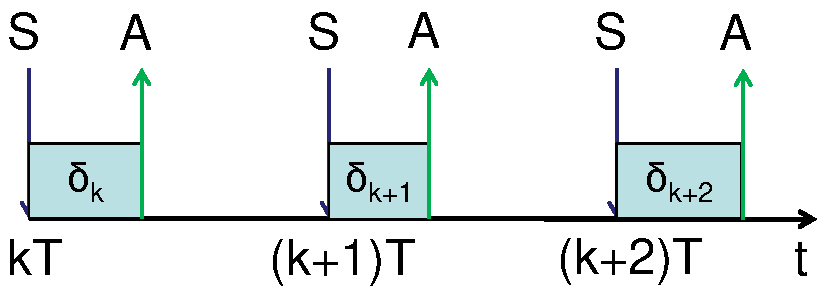
\includegraphics[width=0.45\textwidth,height=24mm]{figs/Timing_Diag.pdf}
	\caption{Timing diagram of Control with Anytime Estimation.  The symbols S and A signify the instants of (periodic) sensing and actuation respectively.}
	\label{fig:timing-diagram}
\end{figure}




\subsection{Discrete-time System Dynamics}

The plant's state at each sampling time $t_{s,k}$ can be described
by the discrete-time system:
\begin{equation}
x_{k+1}=Ax_{k}+B_{1}(\sDelay[k])u_{k-1}+B_{2}(\sDelay[k])u_{k}+w_{k}, k\geq0\label{eq:disc-dynamics} %deleted \qquad from infront of k\geq0
\end{equation}
in which
\begin{gather*}
A=\eu^{A_{c}T}, \quad
w_{k}%=\int_{t_{s,k}}^{t_{s,k+1}}\eu^{A_{c}(t_{s,k+1}-t)}w_{c}(t)\diff t \nonumber \\
=\int_{0}^{T}\eu^{A_{c}(T-t)}w_{c}(t_{s,k}+t)\diff t \\
B_{1}(\sDelay[k])%=\int_{t_{s,k}}^{t_{a,k}}\eu^{A_{c}(t_{s,k+1}-t)}B_{c}\diff t
\!=\!\int_{0}^{\sDelay[k]}\eu^{A_{c}(T-t)}B_{c}\diff t,\,
B_{2}(\sDelay[k])%=\int_{t_{a,k}}^{t_{s,k+1}}\eu^{A_{c}(t_{s,k+1}-t)}B_{c}\diff t
\!=\!\int_{\sDelay[k]}^{T}\eu^{A_{c}(T-t)}B_{c}\diff t \text.
\end{gather*}
Here $w_{k}$ is the accumulated process noise during the interval.
Because $w_{c}(t)$ is constrained in the compact and convex set $\WSet_{c}$
and $T$ is finite, we can find a compact and convex set $\WSet$
that bounds $w_{k}$, namely
\begin{equation}
w_{k}\in\WSet\qquad\forall k\geq0\text{.}\label{eq:disturb-constraint}
\end{equation}
%We remark 
Note that both the current control $u_{k}$ and the previous
control $u_{k-1}$ appear %in the dynamics 
in \eqref{disc-dynamics}.
Furthermore, the input matrices $B_{1}(\sDelay[k])$ and $B_{2}(\sDelay[k])$
depend on the delay $\sDelay[k]$; hence $\sDelay[k]$ is also an
input to the dynamics. The estimation accuracy $\sAccu[k]$ does not
appear in the equation because it only affects the state estimate
$\hat{x}_{k}$ %which is
used by the controller to compute $u_{k}$;
therefore $\sAccu[k]$ indirectly affects the dynamics via the control
input.


\subsection{State and Control Constraints}

For every step $k\geq0$, the actual state of the plant $x_{k}\definedas x(t_{s,k})$
must satisfy a safety condition that 
\begin{equation}
x_{k}\in\XSet\label{eq:state-constraint}
\end{equation}
where $\XSet\subset\RR^{n}$ is the set of safe states. We assume
that $\XSet$ is a polytope of the form $\XSet\definedas\{ x\in\RR^{n}\SuchThat Hx\leq b\} $,
where matrix $H$ and vector $b$ constitute an H-representation
of $\XSet$.
Note that $\XSet$ is not necessarily bounded. In addition, a control
input $u_{k}$ is only valid if it belongs to the predefined set of
admissible control inputs $\USet\subseteq\RR^{m}$ %, that is
\begin{equation}
u_{k}\in\USet\qquad\forall k\geq0\text{.}\label{eq:input-constraint}
\end{equation}
The sets $\XSet$ and $\USet$ are part of the problem statement and
are either chosen by the designer or determined by physical constraints
of the plant and the actuators.


\subsection{Control Performance}

The goal of the controller is two fold: it needs to maintain the state
and control constraints while minimizing a cost function given by
\(
J=\sum_{k=0}^{\infty}\left(\ell(x_{k},u_{k})+\pi(\sDelay[k])\right)
\),
where $\ell(\cdot)$ is the stage cost function for the state and
control, and $\pi(\cdot)$ is the stage cost function for the estimation
and computation.
\begin{comment}
  Typically a longer execution time $\sDelay[k]$ will
  result in a higher computation cost $\pi(\sDelay[k])$. For example,
  if the state estimation involves capturing an image by a camera then
  detecting and locating an object from the image, a longer
  computation time might correspond to a higher resolution of the
  image, more data to be transmitted and processed, and more power
  consumed for communication and computation.
\end{comment}
These stage cost functions are chosen by the designer to achieve a desired control performance.


\subsection{Control Problem}

The control problem is stated as follows.
\begin{problem}\itshape
\label{prob:control-problem}Design a feedback controller, which computes
the admissible control input $u_{k}\in\USet$ and the required estimation
accuracy $\sAccu[k+1]$ (equivalently the delay $\sDelay[k+1]$) based
on the current state estimate $\hat{x}_{k}$, to minimize the cost
$J$ while maintaining the state constraint $x_{k}\in\XSet$ for all
$k\geq 0$.
\end{problem}

\subsection{Notations}

In the rest of this paper, we use the following notational convention.
We write $x_{j\Given k}$ for a variable $x$ at time step $j$ in
the RMPC optimization for time step $k\leq j$ (\ie the prediction
made at time step $k$ of variable $x$ at time step $j$). To emphasize
that this variable depends on an independent variable $v$ we write
$x_{j\Given k}(v)$; however in cases when the dependency is implicitly
understood, we only write $x_{j\Given k}$ for brevity.
We use $\IdentityMatrix_{n}$ to denote the identity matrix of size
$n\times n$. The notation $\bm{0}_{n}$ ($\bm{1}_{n}$) represents
the column vector of length $n$ whose elements are all 0's (respectively
1's). Similarly, $\bm{0}_{n\times m}$ ($\bm{1}_{n\times m}$) is
the matrix of size $n\times m$ whose elements are all 0's (1's).
When the dimensions of the vectors or matrices are obvious
from the context, we drop the subscripts for brevity.

%%% Local Variables: 
%%% mode: latex
%%% TeX-master: "CDC14_Anytime_Main"
%%% End: 
